\section{Исследовательский раздел}

\subsection{Технические характеристики}

Технические характеристики устройства, на котором выполнялось тестирование, следующие:

\begin{itemize}[left=0.49cm, label*=---]
	\item операционная система: Windows 11;
        \item оперативная память: 16 Гб;
	\item процессор: Intel Core™ i5---1135G7.
\end{itemize}

Тестирование проводилось на ноутбуке, который был включен в сеть питания. Во время тестирования ноутбук был нагружен только встроенными приложениями окружения и системой тестирования.


\subsection{Цель и описание исследования}

Целью исследования является исследование зависимости времени выполнения запроса от наличия индексов. 

Исследование проводилось на таблице, содержащих информацию об экспедициях, так как данная таблица является реализацией основной сущности в системе. Для исследования был выбран запрос на поиск всех экспедиций, проведенных в указанной локации. Тестировалось время выполнения запроса при количестве записей в таблице экспедиций от 100 до 10000. Запрос поиска приведен на листинге \ref{res}.

\lstinputlisting[label=res, caption=Запрос поиска]{code/res.sql}

Создание индекса приведено на листинге \ref{index}.

\lstinputlisting[label=index, caption=Создание индекса]{code/index.sql}


Примеры выполнения запроса с индексацией и без представлены на рисунках \ref{img:with-index} и \ref{img:no-index} соответственно.

\begin{figure}[!h]
	\centering
	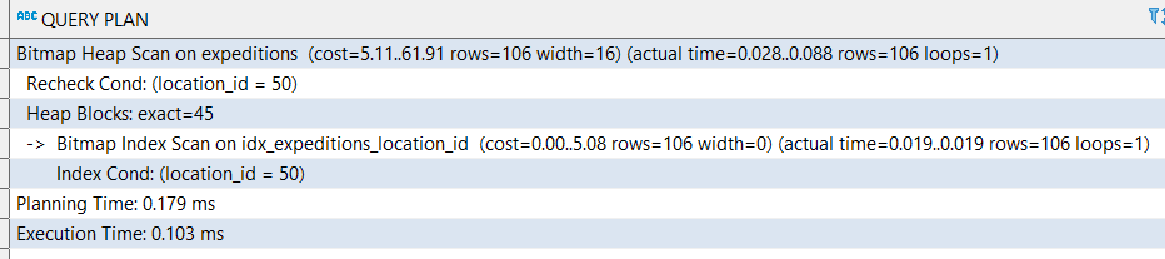
\includegraphics[width=\textwidth]{image/with-index.pdf}
	\caption{Поиск с использованием индексирования}
	\label{img:with-index}
\end{figure}

\begin{figure}[!h]
	\centering
	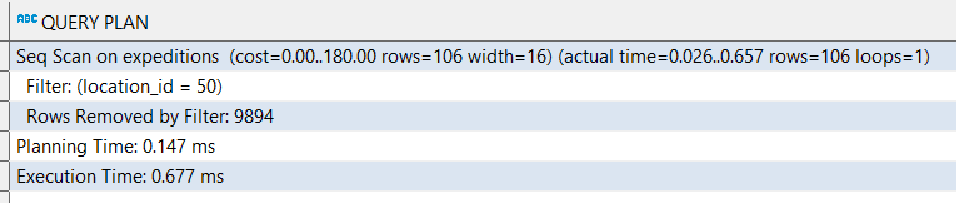
\includegraphics[width=\textwidth]{image/no-index.pdf}
	\caption{Поиск без использования индексирования}
	\label{img:no-index}
\end{figure}

\subsection{Результаты исследования}

График зависимости времени поиска от размера таблицы экспедиций и использования индексирования, представлен на рисунке~\ref{graph}.

\begin{figure}[!h]
	\centering
	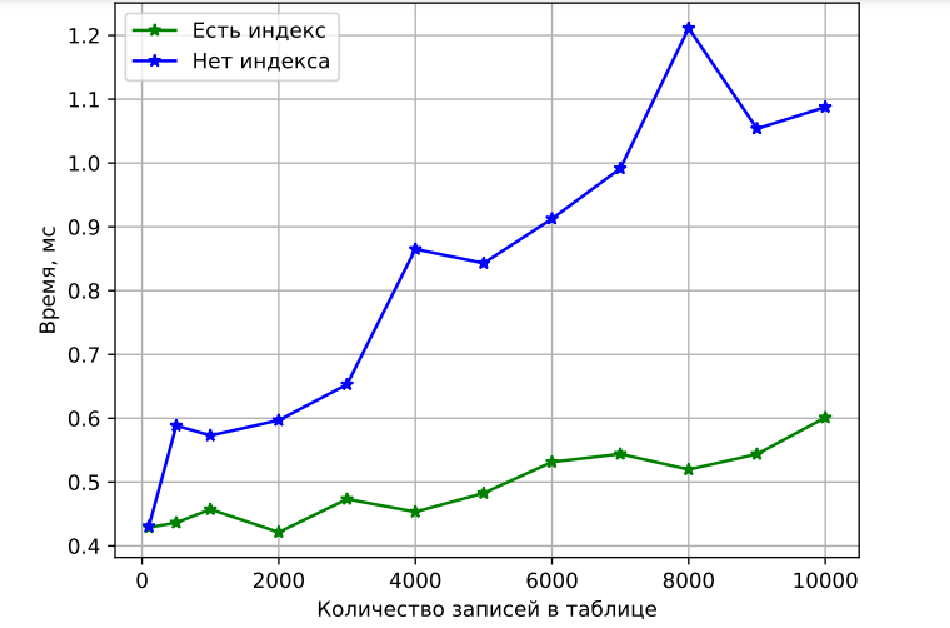
\includegraphics[width=\textwidth]{image/resultGraph}
	\caption{Зависимость времени выполнения поиска от размера таблицы и использования индексирования}
	\label{graph}
\end{figure}
\newpage


\subsection*{Вывод}
В данном разделе было проведено исследование зависимости времени выполнения запроса от наличия индексов.
В результате исследования было выявлено, что использование индексов в среднем уменьшает время выполнения запроса в 1,5---2 раза.
